\documentclass{exam}
\setlength{\parskip}{0pt}
\setlength{\parindent}{0pt}
\setlength{\voffset}{-15pt}
\usepackage[onehalfspacing]{setspace} % Sets Spacing to 1.5
\usepackage[utf8]{inputenc} % Use UTF-8 encoding
\usepackage{float} % Improved interface for floating objects
\usepackage[colorlinks = true,
            linkcolor = blue,
            urlcolor  = blue,
            citecolor = blue,
            anchorcolor = blue]{hyperref} % For hyperlinks in the PDF
\usepackage{graphicx, multicol} % Enhanced support for graphics
\usepackage{amsmath}
\usepackage{framed, caption}
\usepackage{array}
\usepackage{float}
\usepackage{amsmath}
\usepackage{bbm}
\newcommand\tab[1][0.2cm]{\hspace*{#1}}
\usepackage{multicol}
%----------------------------------------------------------------------------------------
\begin{document}

\begin{minipage}{0.295\textwidth} % Left side of title section
\raggedright
SIL765 - Net. \& Sys. Security\\ % Your lecture or course
\footnotesize % Authors text size
CSE, IIT Delhi (SEM2, 2020-21) % Department
\medskip\hrule
\end{minipage}
\begin{minipage}{0.4\textwidth} % Center of title section
\centering 
\large % Title text size
\textbf{Assignment 1}\\ % Assignment number
\normalsize % Subtitle text size
 % Assignment subtitle
\end{minipage}
\begin{minipage}{0.295\textwidth} % Right side of title section
\raggedleft
2018CS10388\\ % Entry Number
\footnotesize
Sharique Shamim % Name
\medskip\hrule
\end{minipage}
\vspace{0.1in}
\section{Birthday Attack}
To run the script do:
\begin{center}
    \texttt{cd problem-2} \\
    \texttt{python3 bithdayattack.py}
\end{center}
A cryptographic hash function is an exceptional class of hash function that has certain properties that make it appropriate for use in cryptography. It is a numerical algorithm that maps information of self-assertive size to a piece line of a fixed size (a hash function) which is intended to likewise be a one-way output function, that is, a function which is infeasible to revert. \vspace{0.05in} \\
To calculate the cryptographic hash value in Python, “hashlib” Module is used. The hashlib gives the following cryptographic hash functions to discover the hash output of a text as follows:
\begin{itemize}
    \item SHA3-224 – 28 bit Digest-Size
    \item SHA3-256 – 32 bit Digest-Size
    \item SHA3-384 – 48 bit Digest-Size
    \item SHA3-512 – 64 bit Digest-Size
\end{itemize}
I have used SHA3-256 for the birthday attack problem.
\begin{framed}
\textbf{Birthday Attack Algorithm}: \vspace{0.05in} \\
def \texttt{birthday\_attack(d):} \vspace{0.05in} \\
\tab log\_dict = \{\} \vspace{0.05in} \\
\tab attempts = 0 \vspace{0.05in} \\
\tab while True: \vspace{0.05in} \\
\tab \tab hash\_num = random.random() \vspace{0.05in} \\
\tab \tab digest = hashlib.sha3\_256(str(hash\_num)).hexdigest() \vspace{0.05in} \\
\tab \tab dbits = hex\_to\_bin(digest)[:d] \vspace{0.05in} \\
\tab \tab if dbits in log\_dict: \vspace{0.05in} \\
\tab \tab \tab return attempts, hash\_num, log\_dict[dbits], digest \vspace{0.05in} \\
\tab \tab log\_dict[dbits] = hash\_num \vspace{0.05in} \\
\tab \tab attempts += 1
\end{framed}
I have computed the tuple (s1, s2, h, m, n) for d = 1 to d = 24. The maximum number of attempts required over all d values is 105 attempts and the maximum memory used over all values of d is 20024 KB. \vspace{0.05in} \\
\textbf{Conclusion}: As the value of d increases i.e the number of bits to be same in the hash output of two strings, the memory used increases and the number of attempts also increase. The values of d asked from us is very small, however in real life it might be large and thus require more memory and attempts to find the collision. In such cases the hash function can be optimized to speedup the process of finding hash output. The following strategy can be used as described here in point 3 \\
\url{https://iopscience.iop.org/article/10.1088/1742-6596/1486/3/032004/pdf}
\begin{figure}[h]
\centering
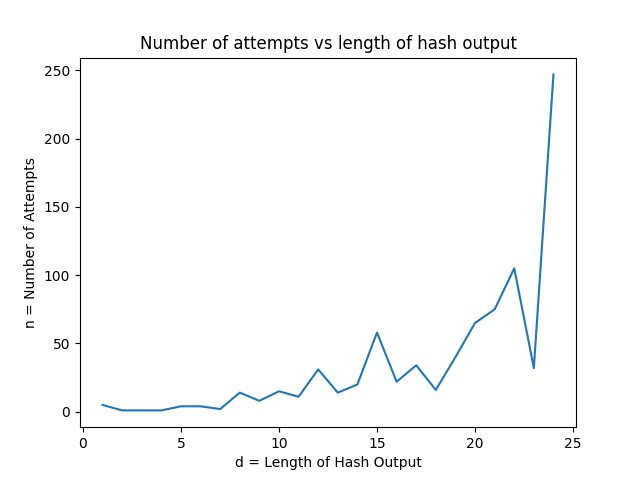
\includegraphics[scale=0.7]{attempts.png}
\end{figure}
\begin{figure}[h]
\centering
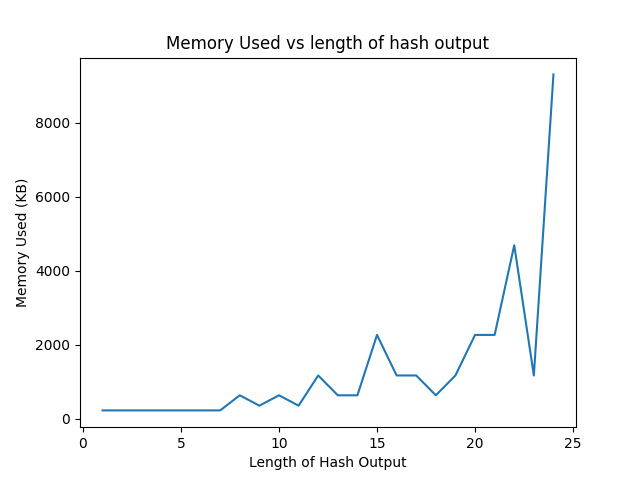
\includegraphics[scale=0.65]{memory.png}
\end{figure}
\end{document}